%-------------------BIBLIOTECAS--------------------
\documentclass[12pt]{report}
\renewcommand{\baselinestretch}{1.5} 
\usepackage[brazil]{babel} 
\usepackage[utf8x]{inputenc} 
%\usepackage[latin1]{inputenc}
\usepackage{graphicx}
\usepackage{wrapfig}
\usepackage{amssymb, amsmath, pxfonts} %permite simbolos matemáticos
\usepackage{indentfirst}%para indentacao
\usepackage{fontspec}%pra a fote no mac

%/~
%\^
\usepackage[left=20mm, right=20mm, bottom=20mm, top=20mm]{geometry}%define a margem do 
\usepackage[colorinlistoftodos]{todonotes}
%\usepackage[style=authoryear]{biblatex}

%-----------------DADOS DO DOCUMENTO---------------------
%\title{Modelagem de Sistema com ModSym}
%\author{Jaime Cristalino Jales Dantas}
%\date{Quinta-feira, 24 de março de 2016}
%\maketitle
%------------------PAGINA DE TITULO-----------------
\begin{document}
\setmainfont{CMU Serif}%pra a fonte no mac
%\usefont{0T1}{cmr}{m}{n}{10} Computer Modern Roman 10 point

%\usefont{0T1}{cmr}{db}{sp} Computer Modern Roman 
\begin{titlepage}

\newcommand{\HRule}{\rule{\linewidth}{0.5mm}} % Defines a new command for the horizontal lines, change thickness here

\center % Center everything on the page
 
%----------------------------------------------------------------------------------------
%	HEADING SECTIONS
%----------------------------------------------------------------------------------------

\textsc{\large\bfseries UNIVERSIDADE FEDERAL DO RIO GRANDE DO NORTE\\}% Name of your university/college
\vspace{4mm}
\textsc{ DEPARTAMENTO DE ENGENHARIA DE COMPUTAÇ\~AO E AUTOMAÇ\~AO\\} % Major heading such as course name
\vspace{4mm}
\textsc{ CURSO DE ENGENHARIA DE COMPUTAÇ\~AO}\\ % Minor heading such as course title
\vspace{4mm}
\textsc{ MODELAGEM E ANÁLISE DE SISTEMAS DINA\̂MICOS}\\ % Minor heading such as course title
\vspace{1cm}
%----------------------------------------------------------------------------------------
%	TITLE SECTION
%----------------------------------------------------------------------------------------

\includegraphics[height=6cm]{Brasao-UFRN} % Include a department/university logo - this will require the graphicx package
 

\HRule \\[0.4cm]
{ \huge \bfseries Modelagem de Sistema com ModSym} % Title of your document
\HRule \\[2.5cm]
 
%----------------------------------------------------------------------------------------
%	AUTHOR SECTION
%----------------------------------------------------------------------------------------

\begin{minipage}{0.45\textwidth}
\begin{flushleft} \large
\emph{Aluno:}\\
Jaime Dantas

\end{flushleft}
\end{minipage}
~
\begin{minipage}{0.4\textwidth}
\begin{flushright} \large
\emph{Professor:} \\
Dr. André Laurindo Maitelli % Supervisor's Name
\end{flushright}
\end{minipage}\\[40mm]


%----------------------------------------------------------------------------------------
%	DATE SECTION
%----------------------------------------------------------------------------------------

{\large \today}\\[2cm] % Date, change the \today to a set date if you want to be precise

%----------------------------------------------------------------------------------------
%	LOGO SECTION
%----------------------------------------------------------------------------------------

%----------------------------------------------------------------------------------------

\vfill % Fill the rest of the page with whitespace

\end{titlepage}
	
%\begin{abstract}
%Your abstract.
%\end{abstract}
\section*{Enunciado do Problema}
\linespread{1.3}

\indent Considere o sistema abaixo, composto de dois motores de corrente contínua com imã permanente (campo constante) conectados a um mesmo corpo através de dois sistemas pinhão-cremalheira e duas molas. O deslizamento das cremalheiras sobre a superfície de apoio acontece praticamente sem atrito. O momento de inércia do pinhão e a massa da cremalheira são desprezíveis. O atrito entre o corpo e a superfície pode ser considerado viscoso. A indutância de armadura dos dois motores é desprezível. Assuma conhecidas as constantes necessárias para modelar o sistema: resistências de armadura $(R_1 e R_2)$, constantes do motor $(K_1 e K_2)$ e momentos de inércia dos rotores $(J_1 e J_2)$ das máquinas, raios $(r_1 e r_2)$ das engrenagens, constantes elásticas $(k_1 e k_2)$ das molas, coeficiente de atrito viscoso (b) entre o corpo e o solo, massa (M) do corpo, etc.\\

\begin{figure}[h]
	\centering
	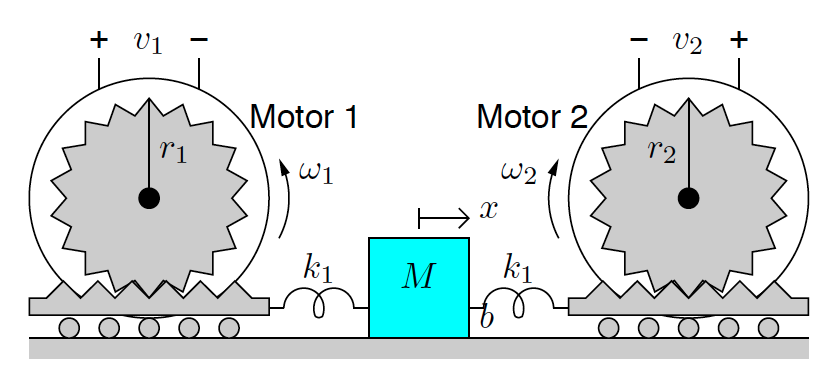
\includegraphics[scale=0.5]{sistema}
	\caption{Sistema Mecânico}
\end{figure}
\newpage
\section*{Modelagem Elétrica do Sistema }
\linespread{1.3}

\indent Foi realizado a modelagem do sistema descrito acima eletricamente. Os componentes mecânicos foram transformados nos seus respectivos componentes elétricos adotando-se o sistema padrão de conversão. Usando-se o ModSym foi modelado o circuito do sistema como apresentado abaixo.

\begin{figure}[h]
	\centering
	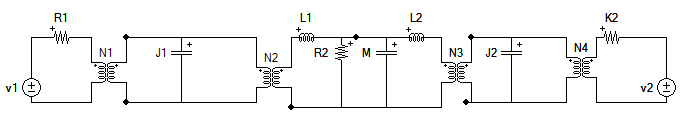
\includegraphics[scale=0.74]{eletrico}
	\caption{Sistema Elétrico}
\end{figure}



\indent Usando o ModSym foi encontrado as função transferências $G_i(s)$ pedido no problema. A equação \ref{eq2}} abaixo representa a função $ H_1(S) = \frac{X(s)}{V_1(s)}$. O $X(s)$ é a tensão sobre o capacitor $M$.


\begin{equation} \label{eq2}
H_1(S) = \frac{Numerador}{Denominador}
\end{equation} 


\indent Onde\


\textbf{Numerador} = (J_2.K_2.L_2.N_1.N_2.N_4^2.R_2)s^2 + (L_2.N_1.N_2.R_2)s + K_2.N_1.N_2.N_3^2.N_4^2.R_2

\begin{multline*}
	
\textbf{Denominador} &= (J_1.J_2.K_2.L_1.L_2.M.N_2^2.N_4^2.R_1.R_2)s^5 + (J_1.J_2.K_2.L_1.L_2.N_2^2.N_4^2.R_1)s^4 + \\(J_1.L_1.L_2.M.N_2^2.R_1.R_2)s^4 + 
	(J_2.K_2.L_1.L_2.M.N_1^2.N_2^2.N_4^2.R_2)s^4 +(J_1.J_2.K_2.L_1.N_2^2.N_4^2.R_1.R_2)s^3 +\\(J_1.J_2.K_2.L_2.N_2^2.N_4^2.R_1.R_2)s^3 + 
(J_1.K_2.L_1.M.N_2^2.N_3^2.N_4^2.R_1.R_2)s^3 + (J_1.L_1.L_2.N_2^2.R_1)s^3 + \\
(J_2.K_2.L_1.L_2.N_1^2.N_2^2.N_4^2)s^3 + 
(J_2.K_2.L_2.M.N_4^2.R_1.R_2)s^3 +
 (L_1.L_2.M.N_1^2.N_2^2.R_2)s^3 + \\(J_1.K_2.L_1.N_2^2.N_3^2.N_4^2.R_1)s^2 + (J_1.L_1.N_2^2.R_1.R_2)s^2 + 
(J_1.L_2.N_2^2.R_1.R_2)s^2 +\\
 (J_2.K_2.L_1.N_1^2.N_2^2.N_4^2.R_2)s^2 +
  (J_2.K_2.L_2.N_1^2.N_2^2.N_4^2.R_2)s^2 + 
  (J_2.K_2.L_2.N_4^2.R_1)s^2 + \\
(K_2.L_1.M.N_1^2.N_2^2.N_3^2.N_4^2.R_2)s^2 +(L_1.L_2.N_1^2.N_2^2)s^2 +
 (L_2.M.R_1.R_2)s^2 + \\
 (J_1.K_2.N_2^2.N_3^2.N_4^2.R_1.R_2)s + 
(J_2.K_2.N_4^2.R_1.R_2)s + (K_2.L_1.N_1^2.N_2^2.N_3^2.N_4^2)s +
 (K_2.M.N_3^2.N_4^2.R_1.R_2)s +\\
  (L_1.N_1^2.N_2^2.R_2)s +
   (L_2.N_1^2.N_2^2.R_2)s + 
   (L_2.R_1)s +
    K_2.N_1^2.N_2^2.N_3^2.N_4^2.R_2 +
     K_2.N_3^2.N_4^2.R_1 + R_1.R_2 



\end{multline*}


\indent A equação \ref{eq2} abaixo representa a função $ H_2(S) =\frac{X(s)}{V_2(s)}$ 

\begin{equation} \label{eq2}
H_2(S) = \frac{Numerador}{Denominador}
\end{equation} 
\indent Onde\

\textbf{Numerador} = (J_1.L_1.N_2^2.N_3.N_4.R_1.R_2)s^2 + (L_1.N_1^2.N_2^2.N_3.N_4.R_2)s + N_3.N_4.R_1.R_2 

\begin{multline*}
	
\textbf{Denominador} &= 
(J_1.J_2.K_2.L_1.L_2.M.N_2^2.N_4^2.R_1.R_2)s^5 + (J_1.J_2.K_2.L_1.L_2.N_2^2.N_4^2.R_1)s^4 + \\(J_1.L_1.L_2.M.N_2^2.R_1.R_2)s^4 + (J_2.K_2.L_1.L_2.M.N_1^2.N_2^2.N_4^2.R_2)s^4 + (J_1.J_2.K_2.L_1.N_2^2.N_4^2.R_1.R_2)s^3 + \\(J_1.J_2.K_2.L_2.N_2^2.N_4^2.R_1.R_2)s^3 + 
(J_1.K_2.L_1.M.N_2^2.N_3^2.N_4^2.R_1.R_2)s^3 + 
(J_1.L_1.L_2.N_2^2.R_1)s^3 +\\
 (J_2.K_2.L_1.L_2.N_1^2.N_2^2.N_4^2)s^3 +
  (J_2.K_2.L_2.M.N_4^2.R_1.R_2)s^3 +
   (L_1.L_2.M.N_1^2.N_2^2.R_2)s^3 +\\
    (J_1.K_2.L_1.N_2^2.N_3^2.N_4^2.R_1)s^2 +
     (J_1.L_1.N_2^2.R_1.R_2)s^2 +
      (J_1.L_2.N_2^2.R_1.R_2)s^2 +\\
       (J_2.K_2.L_1.N_1^2.N_2^2.N_4^2.R_2)s^2 +
        (J_2.K_2.L_2.N_1^2.N_2^2.N_4^2.R_2)s^2 +
         (J_2.K_2.L_2.N_4^2.R_1)s^2 +\\
          (K_2.L_1.M.N_1^2.N_2^2.N_3^2.N_4^2.R_2)s^2 +
           (L_1.L_2.N_1^2.N_2^2)s^2 + 
           (L_2.M.R_1.R_2)s^2 +\\
            (J_1.K_2.N_2^2.N_3^2.N_4^2.R_1.R_2)s +
             (J_2.K_2.N_4^2.R_1.R_2)s +
(K_2.L_1.N_1^2.N_2^2.N_3^2.N_4^2)s +\\
 (K_2.M.N_3^2.N_4^2.R_1.R_2)s + 
 (L_1.N_1^2.N_2^2.R_2)s + 
 (L_2.N_1^2.N_2^2.R_2)s +
  (L_2.R_1)s + \\
  K_2.N_1^2.N_2^2.N_3^2.N_4^2.R_2 + 
  K_2.N_3^2.N_4^2.R_1 +
   R_1.R_2 

\end{multline*}



\indent Por limitações do sistema ModSym não foi possível inserir valores fracionários literais para as resistências, indutores e transformadores do sistema. As relações apresentadas abaixo representam as equivalências do sistema. Para a relação dos tranformadores, o valor apresentador já é a relação de $\frac{N_{primario}}{N_{secundario}}$ como apresentado na equação \ref{eq3}, que representa o ganho do transformador.

\begin{equation} \label{eq3}
i_2 = N_k*i_1\\
\textit{ ,  onde  } N_k = \frac{N_{primario}}{N_{secundario}}
\end{equation}

\newpage
%\hline \\[1cm]
	\hline
	\hline


\textbf {\\Transformadores (Expresso em função de seu respectivo ganho $N_k$):}\\
	\begin{center}
	$N_1=\frac{k_1}{L}$\\ 
	$N_2=\frac{L}{r_1}$ \\
	$N_3=\frac{r_2}{L}$ \\
	$N_4=\frac{L}{k_2}$
	\end{center}
\hline
\hline

\textbf {\\Resistores:}
	\begin{center}
	$R_2=\frac{1}{b}$\\ 
	\end{center}
	\hline
	\hline

\textbf {\\Indutores:}
	\begin{center}
	$L_1=\frac{1}{K_1}$\\ 
	$L_2=\frac{1}{K_2}$ 
	\end{center}
	\hline
	\hline
\indent \\

\indent Por fim, devemos observar é que a função transferência $G(s)$ que queremos encontrar para os dois casos descritos acima está relacionada com a função $H(s)$ encontrada como mostrado na equação \ref{eq4} abaixo.

\begin{equation} \label{eq4}
G(s) = \frac{1}{s} * H(s)
\end{equation}
%-----------------------BIOGRAFIA-----------------------------------------

\begin{thebibliography}{unsrt}

\bibitem{artigo}
  Maitelli, André Laurindo 
  \emph{\bfseries Modelagem e Análise de sistemas Dinâmicos},
  Universidade Federal do Rio Grande do Norte, julho de 2010. 
  Acesso em 5 de maio de 2016.
  
  
\bibitem{artigo}
  Maitelli, André Laurindo 
  \emph{\bfseries APOSTILA DE USO DO SOFTWARE COMPUTACIONAL ModSym},
  Universidade Federal do Rio Grande do Norte, Abril de 2008. 
  Acesso em 5 de maio de 2016.
  
%\citeindextrue

\end{thebibliography}




\end{document}

















